\chapter{RBF-FD method}

%TODO: Valuta se mettere i 2 punti davanti gli uguale quando definisci qualcosa facendolo cadere dall'alto

In this chapter we explain in more details the Meshless Method (MM) used within this work: the Radial Basis Function generated Finite Differences (RBF-FD) method.
To do so we show how it can be used to solve the general boundary value problem defined in chapter~\ref{chap:meshless_methods}.
From now on, in order to be able to discretize the PDE, we consider to have a disposal a set of $N$ distinct nodes, $\mathcal{X}$, defined as follow:
\begin{equation}
\label{eqn:generic_set_of_nodes_X}
	\mathcal{X} := \Set{\vec{x}_1, \dots, \vec{x}_N \mid \vec{x}_i \in \Omega\cup\partial\Omega, \, i=1, \dots, N}
\end{equation}
where $\Omega\cup\partial\Omega \subset \R^d$ is the physical domain of the problem, $\Omega$ and $\partial\Omega$ indicate respectively its open subset and boundary, and $d \in \N$ is its dimension.

%TODO: Fai due parole sulcome vengono disposti i nodi sul dominio



\section{Scattered Data Interpolation}
\label{sec:scattered_data_interpolation}

Every MM, as we have already seen, on its core, is just a way to approximate the solution of a PDE and RBF-FD method is no exception; the tool used to do so is called \emph{scattered data interpolation}. In this section we first see what scattered data interpolation is and then how it is related to PDEs solution. In the second part of the explanation we see how it is applied in general by MMs so to avoid to becoming fixated on a single implementation and losing generality; moreover this approach is still useful since it establishes all the steps that are also followed by RBF-FD.
To avoid from the very beginning any kind of ambiguity we underline that scattered data interpolation is inherently connected to data fitting and not to PDEs approximation, consequently, it finds many other applications beyond the realm of MMs. Examples of its application on the field of image processing can be found in~\cite{Amidror:scattered_data_interpolation_in_image_processing}.

\smallskip
In general the interpolation problem has the following, simple, formulation. Given:
\begin{itemize}
	\item a finite set of nodes,  $\mathcal{X} \subset \R^d$, which can be the one reported in~\eqref{eqn:generic_set_of_nodes_X} and;
	\item a set of known real values $u(\vec{x}_1), \dots, u(\vec{x}_N)$, which may be obtained from a function
\end{itemize}
we want to find a continuous function $u^{h} \colon \Omega\cup\partial\Omega\subset\R^{d} \to \R$ that satisfy:
\begin{equation}
	\label{eqn:interpolation_constraints}
	u^{h}(\vec{x_i}) = u(\vec{x}_i) \qquad  \forall \vec{x}_i \in \mathcal{X}
\end{equation}
If the locations, the nodes in $\mathcal{X}$ where the measurements $u(\vec{x}_1), \dots, u(\vec{x}_N)$ are taken, are placed on a uniform or regular grid we talk about interpolation, otherwise the process above is called \emph{scattered} data interpolation. Here the main idea is to find a function $u^h$ which is a ``good''  fit to the given data, where with ``good'' we mean a function that exactly match the given measurements at the corresponding locations.

MMs also aim to provide an approximation for an unknown function defined as a linear combination of a set of basis functions as reported in equation~\eqref{eqn:general_u_discretization}; we report here for clarity its definition:
\begin{equation}
	\label{eqn:general_u_discretization_RBF_section}
	u^{h}({x}) = \sum_{k= 1}^{N} {\alpha_k B_k(\vec{x})}
\end{equation}
and we remark that coefficients $\alpha_k$ are unknown.
Here is where the theory of scattered data interpolation is applied: it tells us that we are able to find the numerical values for $\alpha_1, \dots \alpha_N$ if we impose a number of conditions equal to the number of coefficients that we are looking for. These conditions must have a form like that shown in equation~\eqref{eqn:interpolation_constraints}. Therefore if we replace the generic meshless approximation within each of the $N$ interpolation conditions we can write the following linear system:
\begin{equation}
	\label{eqn:general_system_from_scattred_data_interpolation}
	\underbrace{
		\begin{bmatrix}
			B_1(\vec{x}_1)  & \dots		& B_N(\vec{x}_1)     \\
			\vdots					& \ddots  & \vdots					      \\
			B_1(\vec{x}_N)  & \dots		& B_N(\vec{x}_N)
	\end{bmatrix}}_{\boldsymbol{B}}
	\begin{bmatrix}
		\alpha_1 \\
		\vdots		\\
		\alpha_N
	\end{bmatrix}
	=
	\begin{bmatrix}
		u(\vec{x}_1)  \\
		\vdots				\\
		u(\vec{x}_N)
	\end{bmatrix}
\end{equation}
that, once solved, provides us the desired coefficients that uniquely define $ u^h $ given the set of basis functions $ \Set{B_1, \dots, B_N} $.
We would like to stress the fact that, however, the right hand side vector is made up of values of the unknown exact solution of problem~\eqref{eqn:generic_continous_PDE}.

\medskip
During the solution of problem~\eqref{eqn:generic_continous_PDE}, via Collocation Methods, the following constraints arise instead:
\begin{equation}
	\begin{aligned}
		\mathcal{L} u^h(\vec{x}_j) = f(\vec{x}_j) \quad & \text{if $\vec{x}_j \in \Omega$}  \\
		u^h(\vec{x}_j) = g(\vec{x}_j) 						    \quad & \text{if $\vec{x}_j \in \partial\Omega$}
	\end{aligned}
\end{equation}
and if we arrange the nodes such that the first $N_I$ nodes belongs to $\Omega$ and the last $N_B$ to $\partial\Omega$, we can find the values of the approximated solution at the points in $\mathcal{X}$ by solving:
\begin{equation}
	\begin{bmatrix}
		c_{1,1} 		& 	\dots 		& c_{1,N_I}  \\
		\vdots			& \ddots	& \vdots		\\
		c_{N_I,1} & \dots		& c_{N_I,N_I}
	\end{bmatrix}
	\begin{bmatrix}
		u^h(\vec{x}_1)  \\
		\vdots					\\
		u^h(\vec{x}_{N_I})
	\end{bmatrix}
	=
	\boldsymbol{f} -
	\begin{bmatrix}
		c_{1,N_I+1} 		& 	\dots 		& c_{1,N_B}  \\
		\vdots			& \ddots	& \vdots		\\
		c_{N_I,N_I+1} & \dots		& c_{N_I,N_B}
	\end{bmatrix}
	\boldsymbol{g}
\end{equation}
where $\boldsymbol{f} = [f(\vec{x}_1) \dots f(\vec{x}_{N_I})]^T$ and $\boldsymbol{g} = [g(\vec{x}_{N_I+1}) \dots g(\vec{x}_{N_B})]^T$, and the coefficient matrix $\boldsymbol{C}$ is found as the solution of:
\begin{equation}
	\label{eqn:generic_discretized_PDE_by_MMs}
	\begin{bmatrix}
		c_{1,1} 		& 	\dots 		& c_{N_I,1}  \\
		\vdots			& \ddots	& \vdots		\\
		c_{1,N} & \dots		& c_{N_I,N}
	\end{bmatrix}
	=
	\boldsymbol{B}^{-T}
	\begin{bmatrix}
		\mathcal{L} B_1(\vec{x}_1)  & \dots		& \mathcal{L} B_1(\vec{x}_{N_I})     \\
		\vdots												& \ddots  & \vdots					      								  \\
		\mathcal{L} B_N(\vec{x}_1)  & \dots		& \mathcal{L} B_N(\vec{x}_{N_I})
	\end{bmatrix}
\end{equation}
Analyzing each row $\boldsymbol{c}_i = [c_{i,1}, \dots c_{i,N}]$ of matrix $\boldsymbol{C}$ we can notice that are computed solving the following linear systems:
\begin{equation}
	\boldsymbol{B}^T c_i = 
	\begin{bmatrix}
		\mathcal{L} B_1(\vec{x_i})  \\
		\vdots											  \\
		\mathcal{L} B_N(\vec{x_i})
	\end{bmatrix}
	\qquad i=1, \dots, N_I
\end{equation}
which are closely related to the ones obtained from scattered data interpolation reported in~\eqref{eqn:general_system_from_scattred_data_interpolation} due to the presence of the same matrix $\boldsymbol{B}$. We conclude by commenting that equation~\eqref{eqn:generic_discretized_PDE_by_MMs} with matrix $\boldsymbol{B}$ defined as in~\eqref{eqn:general_system_from_scattred_data_interpolation} holds true only in case of Dirichlet boundary conditions, otherwise $\boldsymbol{B}$ would take on a different form.



\section{The Mairhuber-Curtis theorem}
\label{sec:Mairhubert-Curtis}

From the previous discussion, in particular from equation~\eqref{eqn:generic_discretized_PDE_by_MMs}, it can be noticed that matrix $\boldsymbol{B}$ has to be non singular in order to be able to solve the linear system associated to the boundary value problem, and this must hold for each node placement $\mathcal{X}$ (to be read as every possible discretization of the problem domain) as long nodes are distinct. This property of $\boldsymbol{B}$ turns out to be dependent on the choice of the particular set of basis functions: for example if we assume $B_k(\vec{x})\in\Pi_P^d$ and $\Set{B_1(\vec{x}), \dots, B_N(\vec{x})}$ to be a polynomial basis of the space $\Pi_P^d$ of polynomials of degree at most $P$ in $\R^d$, then we are not able to guarantee that $\vec{B}$ is invertible for $d>1$.

This issue is explained in more detail by the Mairhuber-Curtis theorem~\cite{Mairhuber:interpolation_basis_problem}; when dealing with the multidimensional case it is possible to continuously move two nodes along a closed path $P$, that does not interfere with any other node in $\mathcal{X}$, such that they end up by interchanging their original positions without one crossing the path of the other. In the event that these two are the only nodes of $\mathcal{X}$ that are moved, $\boldsymbol{B}$ ends up with two rows exchanged leading to a change in the sign of its determinant, and, since the determinant is a continuous function, this means that there is a moment when the latter vanishes making the matrix singular.

The inconvenience arises from the fact that the set of basis functions is independent from the node position and could be solved by simply choosing a basis that is function of nodes position. By doing so we no more fall in the case of the Mairhuber-Curtis theorem since whenever we move nodes also the base itself changes and if two nodes switches their positions not only their respective rows in $\boldsymbol{B}$ are switched, but also their columns, forcing the determinant not to change in sign.

%TODO: Say something about the suitable node generation algorithm and then tells about polynomial augmentation and why it is required (see Riccardo thesis?). Once you've done that you can continue and start talking about RBF.  DELETE



\section{Radial Basis Functions}
\label{subsec:radial_basis_functions}

Up to now, when talking about the approximated solution of the PDE, $u^h$, we have not specified the type of basis functions which define it. However these must be done in order to be able to find the coefficients $\alpha_k$ in equation~\eqref{eqn:general_u_discretization_RBF_section} and thus its numerical values; furthermore it would be appropriate to select a set of functions that allow the avoidance of the aforementioned Mairhuber-Curtis' theorem case. In this section we will define the ones used by the RBF-FD method: the Radial Basis Functions (RBFs).

RBFs are defined as:
\begin{equation}
	\label{eq:RBF_definition}
	\Phi(\vec{x}, \vec{x}_k) = \varphi(\norm{\vec{x} - \vec{x}_k}_2)
\end{equation}
where $\vec{x}_k \in \R^d$ is a given and known point , $\norm{\cdot}_2$ is the euclidean distance and $\varphi\colon \R \to \R$, named \emph{basic} function, is a (univariate) function which takes the radius $r_k = \norm{\vec{x} - \vec{x}_k}_2$ as input and it is used as generator for all the (multivariate) \emph{basis} functions associated to different $\vec{x}_k$.

Sometimes the notations $\Phi(\vec{x} - \vec{x}_k)$ or $\Phi_k({\vec{x}})$ are also used instead of $\Phi(\cdot, \vec{x}_k)$ where ``$\cdot$'' act as a placeholder for the corresponding argument meaning that varies freely. However the $2$-arguments notation makes clear that $\Phi(\cdot, \cdot)$ is a real valued function defined on the space given by the Cartesian product $\Omega \times \Omega$. This type of functions, in accordance with the definition given in~\cite{Schaback:Kernel_definition}, are called \emph{kernels}. In general at different basic functions $\varphi$ are associated different kernels; some of these are reported in table~\ref{tab:basic_functions}.

\begin{table}
	\caption{Examples of basic functions where $r$ is a real number greater than or equal to zero, and $\epsilon$, called shape factor, is a suitable parameter}
	\label{tab:basic_functions}
	\centering
	\begin{tabular}{cc}
		\toprule
		Name										&  $\varphi(r)$																	\\
		\midrule
		Multiquadratic					 			&  $\sqrt{1+(\epsilon r)^2}$													\\
		Inverse multiquadratic	 					&  $\big(  \sqrt{1 + (\epsilon r)^2}  \big)^{-1}$  								\\
		Thin plate splines			   				&  $r^{2l} \log l, \, l\in\N$													\\
		Gaussian							    	&  $e^{- (\epsilon r)^2}$												  		\\
		Polyharmonics								&  $r^{2l + 1}, \, l\in\N$														\\
		\bottomrule
	\end{tabular}
\end{table}

To further clarify the RBFs name we can notice that they are called:
\begin{description}
	\item[Radial] since the value of each $\Phi(\cdot, \vec{x}_k)$ at each point $\vec{x}$ depends only on the distance between that point and $\vec{x}_k$ through $\norm{\cdot}_2$. Basically they satisfy radial symmetry, i.e. $\Phi(\vec{x}_i, \vec{x}_j) = \Phi(\vec{x}_j, \vec{x}_i)$ for any $\vec{x}_i, \vec{x}_j \in \R^d$;
	\item[Basis] since in case of a set of $N$ distinct nodes in $\R^d$, as can be $\mathcal{X}$ given in~\eqref{eqn:generic_set_of_nodes_X}, the set of radial functions $\Phi_k{(\vec{x})}$ with $k=1, \dots, N$ associated to each point of the set, form a basis for the space of functions:
	\[
	F_{\Phi} := \Set{ \sum_{k=1}^{N} \alpha_k \Phi_k{(\vec{x})},  \quad \alpha_k \in\R, \, \vec{x}_k \in \mathcal{X}}
	\]
\end{description}

In case of RBF-FD method the implementation of scattered data interpolation and the solution of governing equation remain the same as explained in the previous section and leads to a symmetric matrix $\boldsymbol{B}$ defined as:
\begin{equation}
	\boldsymbol{B} =
	\begin{bmatrix}
		\Phi(\vec{x}_1, \vec{x}_1)  & 	\dots 	& 	\Phi(\vec{x}_1, \vec{x}_N)  \\
		\vdots											& \ddots &  \vdots											  \\
		\Phi(\vec{x}_N, \vec{x}_1)  & 	\dots 	& 	\Phi(\vec{x}_N, \vec{x}_N)
	\end{bmatrix}
\end{equation}

We conclude by observing that this functions are particularly convenient since they depend on nodes position through $\vec{x}_k$, thus they allow to avoid the non-invertibility of matrix $\vec{B}$ in case of singular node arrangements (Mairhuber-Curtis theorem).



\section{Polynomial augmentation}
\label{sec:poly_augmentation}

Setting aside the issue of the invertibility of matrix $\boldsymbol{B}$ in case of particular nodes arrangement discussed in previous subsection, we should also take into account  the accuracy of the interpolation that we are able to achieve, which also depends upon the type of functions that we are supposed to approximate.
Indeed RBFs approximation schemes alone are not able to exactly interpolate (i.e. with an accuracy only depending on roud-off errors) constant, linear or higher degree polynomials fields. This is an issue in different important engineering applications such as modeling of constant strain in elastic bodies and steady temperature fields in differentially heated walls~\cite{Zamolo:phd_thesis}.

To overcome this limitation, a polynomial augmentation of degree $P$ is required, leading to the overall formulation for the RBF interpolant:
\begin{equation}
	\label{eqn:RBF_interpolator_plus_polynomial_augmentation}
	u^h(\vec{x}) = \sum_{j=1}^{N} \alpha_j \Phi_j(\vec{x}) + \sum_{k=1}^{M} \beta_k p_k(\vec{x})
\end{equation}
where $M=\binom{P+D}{D}$ is the number of polynomial basis functions with degree $P \le D$, $\Set{p_1(\vec{x}) \dots p_M({\vec{x}})}$ is a complete polynomial basis of $\Pi_P^d$ and $\beta_j$ are the corresponding coefficients. An example of polynomial basis for polynomials of degree $P=1$ in $2D$ has the following $M=3$ elements: $p_1(x,y) = 1$, $p_2(x,y) = x$, $p_3(x,y) = y$.

We must also note that using an interpolant with the introduced polynomial augmentation leads to an underdetermined system in~\eqref{eqn:general_system_from_scattred_data_interpolation}. In order to obtain a square $\vec{B}$ and thus having a solvable system, the following orthogonality conditions have to be imposed:
\begin{equation}
	\label{eqn:orthogonality_conditions_for_square_B_in_case_of_poly_augmentation}
	\sum_{i=1}^{N} \alpha_i p_k(\vec{x}_i) = 0, \qquad k=1, \dots, M
\end{equation}
The coefficients of $u^h$, which are now composed not only by $\vec{\alpha} = [\alpha_1 \dots \alpha_N]$, but also by $\vec{\beta} = [\beta_1 \dots \beta_M]$, can then be found by solving the following system:
\begin{equation}
\label{eqn:general_system_from_scattred_data_interpolation_poly_augmentation}
\underbrace{
\begin{bmatrix}
	\vec{B}  & \vec{P}  \\
	\vec{P}^T  & \vec{0}
\end{bmatrix}
}_{\vec{M}}
\begin{bmatrix}
	\vec{\alpha}  \\
	\vec{\beta}
\end{bmatrix}
=
\begin{bmatrix}
	\vec{u}  \\
	\vec{0}
\end{bmatrix}
\end{equation}
where:
\begin{equation}
	\begin{aligned}
		\vec{P} & =
		\begin{bmatrix}
			p_0(\vec{x}_1)  & \dots     & p_M(\vec{x}_1)  \\
			\vdots					 & \ddots  & \vdots						\\
			p_0(\vec{x}_N)  & \dots     & p_M(\vec{x}_N)  \\
		\end{bmatrix}  \\[2ex]
		\vec{u} & = [u(\vec{x}_1). \dots u(\vec{x}_N)]
	\end{aligned} 
\end{equation}
From its formulation is easy to understand that the system above is simply the composition of the system in equation~\eqref{eqn:general_system_from_scattred_data_interpolation}, in the first row, with constraints~\eqref{eqn:orthogonality_conditions_for_square_B_in_case_of_poly_augmentation} written in compact form, in the second row.

In practice the addition of polynomial basis to the RBF interpolant let us perfectly fit $u(\vec{x})$ not only on collocation points where we have $u^h(\vec{x}_i)  = u(\vec{x}_i)$, but also across the rest of the domain provided that data $u(\vec{x}_1), \dots, u(\vec{x}_N)$ come from a polynomial of total degree less than or equal to $P$.  Nevertheless this procedure has a side effect: not all set of nodes $\mathcal{X}$ nor all basic functions $\varphi$ leads to a well-posed RBF interpolation with a non singular matrix $M$. We will discuss this limitation in more detail in the next section.



\section{Problem solution}
\label{sec:interpolation_prob_solution}

At the beginning of section~\ref{sec:Mairhubert-Curtis} we mentioned that the system in equation~\eqref{eqn:generic_discretized_PDE_by_MMs} might not be solvable in case of a combination of non-point-dependent basis functions and particular nodes arrangements, but, up to now, we did not discuss in general in which cases the interpolation problem is solvable. In this section we will address this shortcoming.

We start by recalling that, in case of pure RBF interpolant, the system that we aim to solve has the following compact form:
\begin{equation}
	\label{eqn:general_system_from_scattred_data_interpolation_compact_form}
	\vec{B} \vec{\alpha} = \vec{u}
\end{equation}
where $\vec{B}$ is a symmetric matrix.
A positive definite $\vec{B}$ would be sufficient in order to solve the above system and this last property depends on the choice of the basic function $\varphi$ used to define the RBFs. By definition only \emph{strictly} positive definite~\cite{Fasshauer:details_on_basic_functions} $\varphi$ are associated to a positive definite $\vec{B}$ and, this, restrict our choices: of those shown in table~\ref{tab:basic_functions} only Inverse Multiquadratic and Gaussian functions satisfy this requirement. The same attributes of $\varphi$ are also inherited by the associated RBFs $\Phi_k$.

However in previous section we have seen that, beyond the solvability issue, a polynomial augmentation of degree $P$ is beneficial for the accuracy of the interpolant $u^h$. This means that the system that we have to solve, in general, is no more in the form shown in equation~\eqref{eqn:general_system_from_scattred_data_interpolation_compact_form}, but rather in the following:
\begin{equation}
\label{eqn:general_system_from_scattred_data_interpolation_poly_augmentation_compact_form}
\vec{M}
\begin{bmatrix}
	\vec{\alpha}  \\  \vec{\beta}
\end{bmatrix} = 
\begin{bmatrix}
	\vec{u}  \\  \vec{0}
\end{bmatrix}
\end{equation}
In this case the matrix we seek to be positive definite would be $\vec{M}$that we recall being defined as:
\begin{equation}
\label{eqn:global_M_definition}
\vec{M} =
\begin{bmatrix}
	\vec{B}    &  \vec{P}  \\
	\vec{P}^T  &  \vec{0}
\end{bmatrix}
\end{equation}
which is symmetric as well. 
To be such the following conditions have to be met~\cite{Miotti:phd_thesis}:
\begin{enumerate}
	\item basic function $\varphi$ has to be \emph{strictly conditionally} positive definite function of order $P$~\cite{Fasshauer:details_on_basic_functions};  \label{enum:condition_on_basic_functions_for_solvability}
	\item matrix $\vec{P}$ has to be full-rank.  \label{enum:condition_on_P_for_solvability}
\end{enumerate}
The first condition allows a greater freedom on the choice of the basic function, compared to the pure RBF interpolant: in fact, the set of strictly conditionally positive definite functions of order $P$ is a superset of strictly positive definite functions. These functions are defined as those that require a polynomial augmentation of order at least $P-1$ in order to give a non singular $\vec{M}$. Strictly conditionally positive definite functions of order $P$ are also strictly conditionally positive definite of any higher order. This means that, in case $u^h$ include a polynomial augmentation of order $1$, we can also use Multiquadratic, Thin plate splines with $l=0$ and Polyharmonics with $l=1$ (refer again to table~\ref{tab:basic_functions} for their definitions) as basic functions. At this point someone might consider increasing the degree $P$ of the polynomial augmentation up to the theoretical limit for the size of matrix $\vec{P}$, i.e. $M=N$, in order to increase the accuracy of the interpolant. % However doing so results in ill-conditioning and singularity issues related to $\vec{P}$ that, since non-singularity of $\vec{P}$ is a necessary condition for the non singularity of $\vec{M}$, also affect $\vec{M}$.
However doing so results in ill-conditioning and singularity issues related to $\vec{P}$ which in turn will have an impact on the singularity of matrix $\vec{M}$.

Therefore, since we require the non singularity of $\vec{M}$, the second condition has to be satisfied. It can be shown that to have a full-rank $\vec{P}$ the set $\mathcal{X}$, containing the nodes respect to which we are carrying out the interpolation, must be $P$-unisolvent~\cite{Fasshauer:details_on_basic_functions}, where $P$ is the degree of the polynomial augmentation. This dependency of $\vec{P}$'s rank on the node locations should not surprise since the matrix columns consist on the elements of the polynomial basis evaluated at the different points in $\mathcal{X}$, and they are required to be linearly independent.

Given the node generation technique used in this work, a safe rule for a stable implementation (in the sense of a well-posed interpolation problem) of the polynomial augmentation is to respect the inequality $2M \le N$ where $M$ is the number of terms in the polynomial basis and $N$ is the number of nodes in $\mathcal{X}$.



\section{Radial Basis Function generated Finite Differences (RBF-FD)}
\label{sec:RBF-FD}

In this section we are going to discuss in detail how Radial Basis Function generated Finite Differences (RBF-FD) meshless method is used to solve Partial Differential Equations (PDEs). Its first implementation was developed by Kansa in~\cite{Kansa:RBF_1,Kansa:RBF_2}. His approach, that we denote as \emph{global method}, due to its computational inefficiencies (that we are going to reference later on this section), was eventually dropped in preference for the one suggested by Tolstykh in~\cite{Tolstykh:RBF_local}. We will denote the latter as \emph{local method}. In recent years RBF-FD local method has been developed and applied with success~\cite{Bueno:RBF-FD_application_1,Bueno:RBF-FD_application_2,Kosec:RBF-FD_application_3,Kosec:RBF-FD_application_4}.

The goal of both methods is to approximate solutions to PDEs, i.e., to find a function (or some discrete approximation to this function) which satisfies a given relationship between various of its derivatives on some given region of space along with some boundary conditions on the boundary of this domain. In most cases an analytical solution cannot be found.
What RBF-FD methods do is replacing derivatives in the differential equation by Finite Difference (FD) approximations in such a way as to obtain a large algebraic system of equations to be solved in place of the differential equation; this could be easily solved with a computer.


%TODO: Is done via scattered data interpolation as stated in its related section (??)X

\subsection{Finite difference method}
\label{subsec:finite_difference_methods}

%TODO: Cita come avviene l'approssimazione (secondo highlights del libro sulle FD) [Prima di quesa frase, ma non nnecessariamente in questa subsection]
Before tackling the approximation of PDEs solution, we first consider the more basic task of approximating the derivatives of a known function by Finite Difference (FD) formulas based only on values of the function itself at discrete points. Given $u$, in the simplest case a function of one variable assumed to be sufficiently smooth, we want to approximate its derivatives at a given point $\overline{x}$ relying solely on its values at a finite number of points close to $\overline{x}$. In general its $k$-th derivative is approximated by the following FD formula:
\begin{equation}
	\frac{d^k u}{dx^k}\bigg|_{x=\overline{x}} = u^{(k)}(\overline{x}) \approx \sum_{i=1}^{n} c_{i}^{k} u(x_i)
\end{equation}
where $u(x_1), \dots, u(x_n)$ are the function's samples and $c_{1}^{k}, \dots, c_{n}^{k}$, which can be computed in different ways such as the method of undetermined coefficients or via polynomial interpolation~\cite{LeVeque:FD_book}, are called FD weights.

\smallskip
To give a concrete example we could approximate $u'(\overline{x})$ with the following one-sided approximations:
\begin{subequations}
	\begin{align}
		D_+ u(\overline{x}) & = \frac{u(\overline{x}+h) - u(\overline{x})}{h}  \label{eqn:forward_FD_approx}\\
		D_- u(\overline{x}) & = \frac{u(\overline{x}) - u(\overline{x}-h)}{h}  \label{eqn:backward_FD_approx}
	\end{align}
\end{subequations}
for some value of $h$. This is motivated by the standard definition of the derivative as the limiting value of this expression as $h \to 0$. In these cases the same FD weights, $\Set{1/h, - 1/h}$, are associated to function values coming from different samples: $\Set{u(\overline{x}+h), u(\overline{x})}$ for equation~\eqref{eqn:forward_FD_approx} and $\Set{u(\overline{x}), u(\overline{x}-h)}$ for~\eqref{eqn:backward_FD_approx}. Another possibility is to use the centered approximation:
\begin{equation}
	D_0 u(\overline{x}) = \frac{u(\overline{x}+h) - u(\overline{x}-h)}{h} = \frac{1}{2} \bigl( D_+ u(\overline{x}) + D_- u(\overline{x}) \bigr)
\end{equation}

To derive approximations to higher order derivatives, besides the two method mentioned above, is also possible to repeatedly apply first order differences. Just as the second order derivatives is the derivative of $u'$, we can view $D^2u(\overline{x})$, the second order derivative approximant, as being a finite difference of first differences: $D^2 u(\overline{x}) = D_+ D_- u(\overline{x})$ or $D^2 u(\overline{x}) = D_- D_+ u(\overline{x})$. If we use a step size $h/2$ in each centered approximation to the first derivative we could also define $D^2 u(\overline{x})$ as a centered difference of centered differences and obtain:
\begin{equation}
	D^2 u(\overline{x}) = \frac{1}{h} \Biggl( \biggl( \frac{u(\overline{x}+h) - u(\overline{x})}{h} \biggr) - \biggl( \frac{u(\overline{x}) - u(\overline{x}-h)}{h} \biggr) \Biggr)
\end{equation}
where FD weights $\Set{1/h^2, -2/h^2, 1/h^2}$ are associated to $\Set{u(\overline{x}+h), u(\overline{x}), u(\overline{x}-h)}$.

%TODO: Ci manca una frase che fa da collante con il capitolo formulation

\subsection{Mathematical formulation}
\label{subsec:RBF-FD_formulation}

After this very brief introduction to finite difference (FD), we can see how they are generalized to PDEs differential operators by RBF-FD in order to obtain easily solvable linear systems.

We start by recalling that the boundary value problem that we have to solve is defined as:
\begin{equation}
	\label{eqn:boundary_value_problem}
	\begin{cases}
		\mathcal{L} u  = f 		 & \text{in $\Omega$} \\
		\mathcal{B} u   = g	     & \text{on $\partial\Omega$}
	\end{cases}
\end{equation}
where $\mathcal{L}$ and $\mathcal{B}$ are linear operators and its solution $u$ could be approximated by a function $u^h$ defined as reported in equation~\eqref{eqn:RBF_interpolator_plus_polynomial_augmentation}:
\begin{equation}
	\label{eqn:Kansa_interpolan}
	u^h(\vec{x}) = \sum_{j=1}^{N} \alpha_j \Phi_j(\vec{x}) + \sum_{k=1}^{M} \beta_k p_k(\vec{x})
\end{equation}
which holds true all over the domain. Coefficients of the expansions are found by solving equation~\eqref{eqn:general_system_from_scattred_data_interpolation_poly_augmentation}:
\begin{equation}
\underbrace{
	\begin{bmatrix}
		\vec{B}  & \vec{P}  \\
		\vec{P}^T  & \vec{0}
	\end{bmatrix}
}_{\vec{M}}
\begin{bmatrix}
	\vec{\alpha}  \\
	\vec{\beta}
\end{bmatrix}
=
\begin{bmatrix}
	\vec{u}  \\
	\vec{0}
\end{bmatrix}
\end{equation}
In order to streamline the explanation of the procedure we split the set of nodes $\mathcal{X}$ reported in~\eqref{eqn:generic_set_of_nodes_X} into the two following sets:
\begin{subequations}
	\begin{gather}
		\mathcal{X}_I := \Set{\vec{x}_1, \dots, \vec{x}_{N_I} \mid \vec{x}_i \in \Omega, \, i=1, \dots, N_I}  \\
		\mathcal{X}_B := \Set{\vec{x}_{N_{I+1}}, \dots, \vec{x}_{N_B} \mid \vec{x}_i \in \partial\Omega, \, i=N_{I+1}, \dots, N_B}
	\end{gather}
\end{subequations}
where $N_I$ and $N_B$ indicate respectively the number of nodes inside and on the boundary of the physical domain (from the definitions of the two sets it also follows that $N_I+N_B = N$ and $\mathcal{X}_I \cup \mathcal{X}_B = \mathcal{X}$).

The idea that Kansa used to discretize the problem reported above is to use the theory of interpolation to approximate the differential operator $\mathcal{L}$ in the PDE, with an operator $\mathcal{L}^h$ represented by a matrix $\vec{C}_I$, using a FD-like method.
%The data used for the interpolation are $\Set{\mathcal{L}u(\vec{x}_1), \dots, \mathcal{L}u(\vec{x}_{N_I})}$ and are easily obtainable since $f$ is known and $\mathcal{L} u  = f$ in $\Omega$. 
Tolstykh's approach follows the same concept as Kansa's, but adds \emph{stencil} as novelty.

A stencil of $m$ nodes associated to each node $\vec{x}_i \in \mathcal{X}_I$ is defined as the set $\mathcal{X}_i = \Set{\vec{x}_1, \dots, \vec{x}_m} \subseteq \mathcal{X}$ formed by the $m$ nearest neighbors of $\vec{x}_i$; in addition $\mathcal{X}_i$ can be interpreted as the union of $\mathcal{X}_{i,I} = \Set{\vec{x}_1, \dots, \vec{x}_{m_I}}$ and $\mathcal{X}_{i,B} = \Set{\vec{x}_{m_I+1}, \dots, \vec{x}_m}$, respectively the set of its $m_I$ nodes belonging to $\Omega$ and of its other $m_B$ nodes belonging to $\partial\Omega$. An example of stencil could be found in Figure~\ref{fig:2D_stencil}.

\begin{figure}
\centering
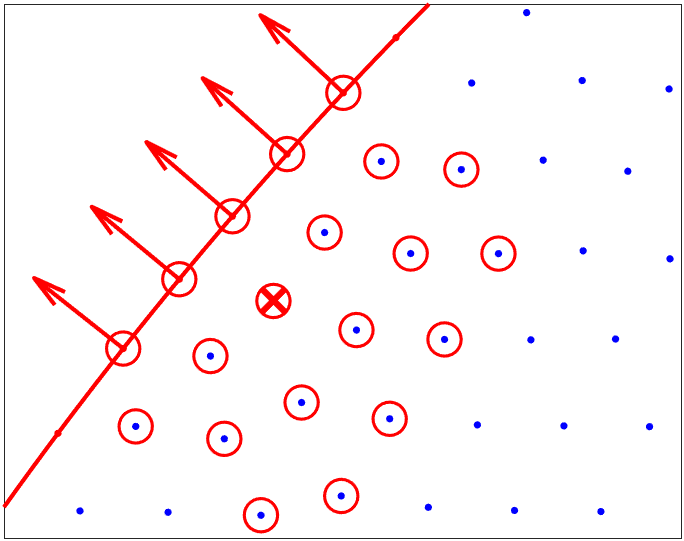
\includegraphics[width=.5\textwidth]{img/2D_stencil}
\caption{Example of $2$D stencil. The nodes which belong to it are marked with a red circle, its central node with a red cross. Red arrows represent the boundary normals $\vec{n}$ of those nodes belonging to $\partial\Omega$. Figure taken from~\cite{Miotti:phd_thesis}} 
\label{fig:2D_stencil}
\end{figure}

%TODO: Add a note that tells that now on we consider only the local method underling the differences with Kansa
In Tolstykh's local method the interpolation scheme is local, i.e. $u^h$ is expanded using a basis that changes depending on the position $\vec{x}$ and it is made valid only inside the stencil centered at $\vec{x}$ rather than globally across the entire domain. Thus, given a point $\vec{x}_i \in \mathcal{X}_I$ along its related stencil $\mathcal{X}_i = \Set{\vec{x}_1, \dots, \vec{x}_m}$, equation~\eqref{eqn:Kansa_interpolan} is rewritten as:
\begin{equation}
	\label{eqn:local_RBF-FD_interpolant}
	u^h(\vec{x}_i) = \sum_{j=1}^{m} \alpha_j \Phi(\vec{x}_i, \vec{x}_j) + \sum_{k=1}^{M} \beta_k p_k(\vec{x}_i)
\end{equation}
In the following, we will focus solely on Tolstykh’s formulation, commonly employed in practice, with a brief mention of Kansa's for comparative purposes.
%TODO: Valuta se mettere il plurale "mentions"

\medskip
Applying operator $\mathcal{L}$ to the definition of $u^h$ results in:
\begin{equation}
	\label{eqn:L_of_local_RBF-FD_interpolant}
	\begin{aligned}
		\mathcal{L} u^h(\vec{x}_i) & = \sum_{j=1}^{m} \alpha_j \mathcal{L} \Phi(\vec{x}_i, \vec{x}_j) + \sum_{k=1}^{M} \beta_k \mathcal{L} p_k(\vec{x}_i)  \\
								   & = \begin{bmatrix}
								   			\vec{\alpha} & \vec{\beta}
								   	   \end{bmatrix}
							   	   	   \begin{bmatrix}
							   	   	   		\mathcal{L} \vec{\Phi}(\vec{x}_i, \mathcal{X}_{i,I})  \\
							   	   	   		\mathcal{L} \vec{p}(\vec{x}_i)
							   	   	   \end{bmatrix}	
	\end{aligned}
\end{equation}
where different vectors of coefficients $\vec{\alpha} = \bigl[\alpha_1, \dots, \alpha_m \bigr] \in \R^m$ and $\vec{\beta} = \bigl[ \beta_1, \dots, \beta_M \bigr] \in \R^M$ are associated to different $\vec{x}_i$.
In order to find them we can note that, since equation~\eqref{eqn:local_RBF-FD_interpolant} is still an approximated solution of the boundary value problem (at least locally), it must satisfy:
%TODO: Valuta se cambiare l'indice da i a j come in tesi Davide pag. 132 oppure ad un altro indice tipo k
\begin{subequations}
\label{eqn:interpolation_conditions_on_PDE}
	\begin{gather}
		u^h(\vec{x}_i) = u(\vec{x}_i) \quad \text{if $\vec{x}_i \in \mathcal{X}_{i,I}$}  \label{eqn:u^h_approx_u_conditions} \\
		\mathcal{B} u^h(\vec{x}_i) = g(\vec{x}_i) \quad \text{if $\vec{x}_i \in \mathcal{X}_{i,B}$} \label{eqn:u^h_approx_conditions_on_boundary}
	\end{gather}
\end{subequations}
which rewritten in matrix form read as:
\begin{equation}
\label{eqn:interpolation_system_of_RBF-FD}
\underbrace{
\begin{bmatrix}
	\vec{\Phi}_I  			 &  \vec{P}_I  			  \\
	\vec{\mathcal{B}\Phi}_B  &  \vec{\mathcal{B}P}_B  \\
	\vec{P}^T				 &  \vec{0}				  \\
\end{bmatrix}}_{\vec{M}_{BC}}
\begin{bmatrix}
	\vec{\alpha}  \\
	\vec{\beta}
\end{bmatrix}
=
\begin{bmatrix}
	\vec{u}_I  \\
	\vec{g}	   \\
	\vec{0}
\end{bmatrix}
\end{equation}
where $\vec{u}_I = \left[ u(\vec{x}_1), \dots, u(\vec{x}_{m_I}) \right]^T \in R^{m_I}$ and $\vec{g} = \left[g(\vec{x}_{m_I+1}), \dots, g(\vec{x}_m)\right]^T \in \R^{m_B}$ and the new terms in $\vec{M}_{BC} \in \R^{(m+M) \times (m+M)}$ are defined as follow:
\begin{equation}
	\begin{gathered}
		\vec{\Phi}_I = \begin{bmatrix}
							\Phi(\vec{x}_1, \vec{x}_1)    	  &    \dots    & \Phi(\vec{x}_1, \vec{x}_m)  		\\
							\vdots						  	  &  \ddots		& \vdots					  		\\
							\Phi(\vec{x}_{m_i}, \vec{x}_1)    &    \dots    & \Phi(\vec{x}_{m_I}, \vec{x}_m)
					   \end{bmatrix} \in \R^{m_I \times m}  \\[2ex]
		\vec{P}_I = \begin{bmatrix}
							p_1(\vec{x}_{1})	&  \dots  &  p_M(\vec{x}_{m_I})   \\
							\vdots				& \ddots  & \vdots					\\	
							p_1(\vec{x}_{1})	&  \dots  &  p_M(\vec{x}_{m_I})
					\end{bmatrix} \in \R^{m_I \times M}  \\[2ex]
		\vec{\mathcal{B}\Phi}_B = \begin{bmatrix}
										\mathcal{B}\Phi(\vec{x}_{m_I+1}, \vec{x_1})  &  \dots  & \mathcal{B}\Phi(\vec{x}_{m_I+1}, \vec{x}_m)  \\
										\vdots										 & \ddots  & \vdots										  \\
										\mathcal{B}\Phi(\vec{x}_{m}, \vec{x_1})  	 &  \dots  & \mathcal{B}\Phi(\vec{x}_{m}, \vec{x}_m)
								  \end{bmatrix} \in \R^{m_B \times m}  \\[2ex]
		\vec{\mathcal{B}P}_B = \begin{bmatrix}
									\mathcal{B}p_1(\vec{x}_{m_I+1})  &  \dots  & \mathcal{B}p_M(\vec{x}_{m_I+1})  \\
									\vdots							 & \ddots  & \vdots							  \\
									\mathcal{B}p_1(\vec{x}_{m})  	 &  \dots  & \mathcal{B}p_M(\vec{x}_{m})
							  \end{bmatrix} \in \R^{m_B \times M}
	\end{gathered}
\end{equation}
When Dirichlet BC are enforced, $\mathcal{B}$ becomes the identity operator in which case $\vec{M}_{BC}$ in equation~\eqref{eqn:interpolation_system_of_RBF-FD} coincides with the matrix $\vec{M}$ of the interpolation system~\eqref{eqn:general_system_from_scattred_data_interpolation_poly_augmentation} defined in section~\ref{sec:poly_augmentation}. In this case the problem is well-posed, regardless of the shape of domain $\Omega$ if the instructions presented in section~\ref{sec:interpolation_prob_solution} are adhered to. However this is no-longer true in case of Neumann or Robin BCs: we are going to tackle this issue in the next section. For the time being, to proceed with the explanation of RBF-FD, we will assume that the problem is always well-posed regardless of the type of BCs applied.

\medskip
Substituting the recently determined $\vec{\alpha}$ and $\vec{\beta}$ into equation~\eqref{eqn:L_of_local_RBF-FD_interpolant} we obtain:
\begin{equation}
	\label{eqn:FD_like_discretization_of_L_middle_step}
	\mathcal{L} u^h(\vec{x}_i) = 
	\begin{bmatrix}
		\vec{u}_I  &  \vec{g}  &  \vec{0}
	\end{bmatrix}
	\vec{M}_{BC}^{-T}
	\begin{bmatrix}
		\mathcal{L} \vec{\Phi}(\vec{x}_i, \mathcal{X}_{i,I})  \\
		\mathcal{L} \vec{p}(\vec{x}_i)
	\end{bmatrix}	
\end{equation}
We might now observe that the last two factors of this last equation are known, thus we can represent their product with a vector $\vec{c}(\vec{x}_i) = \bigl[ \vec{c}_I(\vec{x}_i), \vec{c}_B(\vec{x}_i), \vec{c}_p(\vec{x}_i) \bigr] \in \R^{m+M}$ that can be obtained solving the dual problem:
\begin{equation}
\label{eqn:row_of_C_system}
	\vec{M}_{BC}^T
	\begin{bmatrix}
		\vec{c}_I(\vec{x}_i)  \\
		\vec{c}_B(\vec{x}_i)  \\
		\vec{c}_p(\vec{x}_i)
   \end{bmatrix} = 
	\begin{bmatrix}
		\mathcal{L} \vec{\Phi}(\vec{x}_i, \mathcal{X}_{i,I})  \\
		\mathcal{L} \vec{p}(\vec{x}_i)
	\end{bmatrix}
\end{equation}
where $\vec{c}_I(\vec{x}_i)$, $\vec{c}_B(\vec{x}_i)$ and $\vec{c}_p(\vec{x}_i)$ denote the first $m_I$, the next $m_B$ and the last $M$ elements of $\vec{c}(\vec{x}_i)$ respectively.
Once this is done~\eqref{eqn:FD_like_discretization_of_L_middle_step} can be rewritten as:
\begin{equation}
	\begin{aligned}
		\label{eqn:FD_like_discretization_of_L}
		\mathcal{L} u^h(\vec{x}_i) & = \vec{c}_I(\vec{x}_i)^T \vec{u}_I + \vec{c}_B(\vec{x}_i)^T \vec{g}  \\[2ex]
								   & = \sum_{j=1}^{m_I} c_j(\vec{x}_i) u(\vec{x}_j) + \sum_{k=m_I+1}^{m} c_k(\vec{x}_i)g(\vec{x}_k)
	\end{aligned}
\end{equation}
which is nothing else but the FD-like approximation of $\mathcal{L}u^h$ at point $\vec{x}_i$ with FD weights given by the elements of the vectors $\vec{c}_I(\vec{x}_i)$ and $\vec{c}_P(\vec{x}_i)$.
Finally we remark that, in this specific case, we can write equation~\eqref{eqn:FD_like_discretization_of_L} thanks to the combination of:
\begin{itemize}
	\item the linearity of $u^h$ respect the parameters $\alpha_1, \dots, \alpha_m$ and $\beta_1, \dots, \beta_M$, as can be seen in equation~\eqref{eqn:local_RBF-FD_interpolant}, and;
	\item the linearity of operator $\mathcal{L}$.
\end{itemize}

\medskip
The values of the approximated solution at the $N_I$ nodes of $\mathcal{X}$, i.e. the solution of the PDE, can be finally found by requiring $u^h$ to approximate the exact solution at each of these points:
\begin{equation}
	\mathcal{L}u^h(\vec{x}_i) = \mathcal{L}u(\vec{x}_i) = f(\vec{x}_i)  \quad  \text{if $\vec{x}_i \in \mathcal{X}_{i,I}$}
\end{equation}
which takes the matrix form:
\begin{equation}
\label{eqn:discretized_version_of_PDE_using_RBF-FD}
\vec{C}_I
\begin{bmatrix}
	u^h(\vec{x}_1)  \\
	\vdots			\\
	u^h(\vec{x}_{N_I})
\end{bmatrix}
=
\begin{bmatrix}
	f(\vec{x}_1)  \\
	\vdots		  \\
	f(\vec{x}_{N_I}))
\end{bmatrix}
-
\vec{C}_B
\begin{bmatrix}
	g(\vec{x}_{N_I+1})  \\
	\vdots				\\
	g(\vec{x}_{N})
\end{bmatrix}
\end{equation}
where rows of matrices $\vec{C}_I$ and $\vec{C}_B$ are formed by the elements of the vectors $\vec{c}_I(\vec{x}_i)$ and $\vec{c}_B(\vec{x}_i)$ found by solving solving equation~\eqref{eqn:row_of_C_system} $N_I$ times:
\begin{equation}
	\begin{gathered}
		\vec{C}_I = \begin{bmatrix}
						c_1{(\vec{x}_1)}  	&  \dots  & c_{N_I}(\vec{x}_1)  	\\
						\vdots				& \ddots  & \vdots					\\
						c_1{(\vec{x}_{N_I})}  &  \dots  & c_{N_I}(\vec{x}_{N_I})
					\end{bmatrix} \in \R^{N_I \times N_I}  \\[2ex]
		\vec{C}_B = \begin{bmatrix}
						c_{N_I+1}{(\vec{x}_1)}  	  &  \dots  & c_{N}(\vec{x}_1)  	\\
						\vdots					  & \ddots  & \vdots				\\
						c_{N_I+1}{(\vec{x}_{N_I})}  &  \dots  & c_{N}(\vec{x}_{N_I})
					\end{bmatrix} \in \R^{N_I \times N_B}
	\end{gathered}
\end{equation}
What we just obtained in~\eqref{eqn:discretized_version_of_PDE_using_RBF-FD} is the algebraic system that once solved, in place of the PDE, gives the values of the PDE approximated solution $\Set{u^h(\vec{x}_1), \dots, u^h(\vec{x}_{N_I})}$. In Kansa's global method the process is followed with the same steps as long as the global expansion of equation~\eqref{eqn:Kansa_interpolan} is used to approximate the PDE solution instead of the local expansion of equation~\eqref{eqn:local_RBF-FD_interpolant}.

\bigskip
An important remark has to be done about computational efficiencies of global and local methods since linear system~\eqref{eqn:row_of_C_system} has to be solved at any point $\vec{x}_i \in \mathcal{X}_I$, therefore requiring the inversion of $N_I$ different $\vec{M}_{BC}^T$ matrices. In case of local method each $\vec{M}_{BC}$ has size $(m+M) \times (m+M)$; instead in global method they have size $(N+M) \times (N+M)$ since conditions~\eqref{eqn:interpolation_conditions_on_PDE} must be enforced not only in the stencil, but over the entire domain due to the global nature of the approximated solution. Remembering that the computational cost of factorizing a matrix is at least of $\bigO(n^3)$, where here $n$ denotes the number of rows and columns of the matrix, then local method is computationally advantageous respect the global one.

Another difference between global and local method is that in global method derivative approximation of $u^h$ at point $\vec{x}_i$ depends on the values of $u$ across the entire domain even if derivatives are local properties of functions: this is clearly suboptimal since leads to a matrix $\vec{C}_I$, which represent the discretized differential operator $\mathcal{L}$, that is full even though it should not be in principle. On the contrary, in local method, $\vec{C}_I$ is sparse since in each row $i$ the number of non-zero entries is equal to the number of internal nodes of stencil $\mathcal{X}_I$.

Finally, indicating with $\vec{u}^h = \left[u(\vec{x}_1), \dots, u(\vec{x}_N)\right]$ the vector of the exact solution evaluated at the RBF-FD nodes and with $\vec{u} = \left[u^h(\vec{x}_1), \dots, u^h(\vec{x}_N)\right]$ the approximated solution obtained from RBF-FD method, is possible to show that the solution error $e(N) = \frac{\norm{\vec{u}^h - \vec{u}}}{\norm{\vec{u}}}$ decrease exponentially as the number of nodes $N$ increase in the global approach. In the local approach, conversely, the solution error decreases ``only'' polynomially.

The reason just listed above are those that explain the benefits of stencil introduction and that led to the choice of Tolstykh approach both in this work and within the community of researchers exploring different Meshless Methods.

\bigskip
What we have not covered yet is the computational cost of the stencils creation: if too expensive, it might loose all the benefits of the local approach. In fact this would be the case when using a brute force approach (which require a computational cost of $\bigO(N^2)$ for each $\vec{x}_i$) where all pairwise distances between nodes are computed and then sorted in order to keep just the $m$-nearest neighbors. To avoid this issue more efficient algorithms has to be used. An example of these is the $k$-d tree algorithm~\cite{Bentley:k-d_tree} which require $\bigO(N \log N)$ operations for rearranging the nodes and other $\bigO(N \log N)$ for finding a fixed number of neighbors.

Finally, regarding to the stencil, we note that the effect of its size are still under research: one of the last activities on this regard is the one of Kolar-Požun et al.~\cite{Kolar-Požun:effect_of_stencil_size} where they found that changing stencil's size induce oscillations in both the solution and discretization errors for the Poisson equation.

%TODO: Add note about p-uisolvent stencil (??)



\section{Radial Basis Functions-Hermite Finite Difference (RBF-HFD)}

In previous section we have overlooked a rather important fact for the implementation of the RBF-FD method: the invertibility of matrix $\vec{M}_{BC}$. In fact is always possible, given a stencil containing boundary points on which Neumann or Robin Boundary Conditions (BCs) are applied, to find normal directions associated with them that make the local natrix $\vec{M}_{BC}$ in equation~\eqref{eqn:interpolation_system_of_RBF-FD} singular~\cite{Miotti:phd_thesis}.

Unfortunately, simply avoiding this kind of boundary condition is not an option due to their importance in most boundary value problems of engineering interest.
%TODO: Aggiungi reference ad altri metodi esistenti per risolvere il problema di ill-conditioning (??)
The solution adopted in the present work to avoid this limitation is the so called Radial Basis Functions-Hermite Finite Difference (RBF-HFD).
Within this section we present the formulation of the aforementioned method after explaining the Hermite interpolation framework which is at its core.


\subsection{Hermite Interpolation}

In the RBF-FD method, to find the approximated solution $u^h$ valid for a given stencil $\mathcal{X}_q = \Set{\vec{x}_1, \dots, \vec{x}_m} \subseteq \mathcal{X}$, based on a point $\vec{x}_q \in \Omega$, the following interpolation conditions are enforced:
\begin{subequations}
	\label{eqn:interpolation_conditions_on_PDE_Hermite_Interpolation_subsection}
	\begin{gather}
		u^h(\vec{x}_i) = u(\vec{x}_i) \quad \text{if $\vec{x}_i \in \mathcal{X}_{q,I}$}  \label{eqn:u^h_approx_u_conditions_RBF-HFD_section} \\
		\mathcal{B} u^h(\vec{x}_i) = g(\vec{x}_i) \quad \text{if $\vec{x}_i \in \mathcal{X}_{q,B}$} \label{eqn:u^h_approx_conditions_on_boundary_RBF-HFD_section}
	\end{gather}
\end{subequations}

In general the action of evaluating a function $u$ at a point $\vec{x}_i$ could be seen as the application of an operator $\delta_{\vec{x}_i}$, called point-evaluation functional, such that $\delta_{\vec{x}_i} u = u(\vec{x}_i)$. Furthermore functional $\delta_{\vec{x}_i}$ can be combined with other operators; an example of this can be found when Neumann BC are encountered in conditions~\eqref{eqn:u^h_approx_conditions_on_boundary_RBF-HFD_section}:
\begin{equation}
	\begin{aligned}
		\mathcal{B} u^h(\vec{x}_i) & = \frac{\partial}{\partial \vec{n}} u^h(\vec{x}_i)											\\
								   & = \bigg( \delta_{\vec{x}_i} \circ \frac{\partial}{\partial \vec{n}} \bigg) u^h(\cdot)
	\end{aligned}
\end{equation}
where $\vec{x}_i$ belongs to $\mathcal{X}_{q,B_N} \subseteq \mathcal{X}_{q,B}$, the set of stencil's boundary nodes on which are applied Neumann BCs. To avoid excessive notation complexity in the following we assume that only Neumann BC are enforced on the points of the stencil that belongs to the boundary of the physical domain, i.e. $\mathcal{X}_{q,B_N} \equiv \mathcal{X}_{q,B}$.

Leveraging on these operators, interpolation conditions, more generally, can be defined through a set of given values $\Set{u(\vec{x}_1), \dots, u(\vec{x}_{m})}$ along with a given set of functionals $\Lambda = \Set{\lambda_1, \dots, \lambda_{m}}$ as follow:
%Leveraging on these operators, interpolation condition, more generally, can be seen as a set of given values $\Set{u(\vec{x}_1), \dots, u(\vec{x}_{m})}$ along with a given set of functionals $\Lambda = \Set{\lambda_1, \dots, \lambda_{m}}$ such that:
\begin{equation}
	\label{eqn:Hermite_interpolation_conditions}
	\lambda_i u^h = \lambda_i u \qquad i = 1, \dots, m
\end{equation}
These conditions are typically called Hermite interpolation conditions~\cite{Fasshauer:details_on_basic_functions}.
For RBF-FD local constraints~\eqref{eqn:interpolation_conditions_on_PDE_Hermite_Interpolation_subsection} we have that $\lambda_i = \delta_{\vec{x}_i}$ for those nodes $\vec{x}_i$ that belong to $\mathcal{X}_{q,I}$ and $\lambda_i = \delta_{\vec{x}_i} \circ \frac{\partial}{\partial \vec{n}}$ for those which belong to $\mathcal{X}_{q,B}$.

\smallskip
In case of pure RBF interpolation scheme the local approximated solution $u^h$ is given by:
\begin{equation}
	\label{eqn:basic_pure_RBF_interpolant}
	u^h(\cdot) = \sum_{j=1}^{m} \alpha_j \Phi(\cdot,\vec{x}_j)
\end{equation}
where ``$\cdot$'' is a placeholder for the argument of the function meaning that it is not evaluated at any point. In this case the basis used for the interpolation is determined solely by the points of the stencil and is given by $\Set{\Phi(\cdot,\vec{x}_1), \dots, \Phi(\cdot,\vec{x}_m)} = \Set{\delta_{2,\vec{x}_1}\Phi(\cdot,\cdot), \dots, \delta_{2,\vec{x}_m}\Phi(\cdot,\cdot)}$ where the subscript $2$ in the point-evaluation functional indicates that it is acting on the second argument of $\Phi(\cdot, \cdot)$. Using interpolant~\eqref{eqn:basic_pure_RBF_interpolant} in case of Hermite interpolation conditions and repeating the same scattered data interpolation procedure described in section~\ref{sec:scattered_data_interpolation}, we would obtain a matrix $\vec{B}$:
\begin{equation}
	\label{eqn:unsymmetric_B}
	\vec{B} = 
	\begin{bmatrix}
		\lambda_1 \Phi(\vec{x}_1, \vec{x}_1)  &  \dots  & \lambda_1 \Phi(\vec{x}_1, \vec{x}_m)  \\
		\vdots								  & \ddots	& \vdots								 \\
		\lambda_m \Phi(\vec{x}_m, \vec{x}_1)  &  \dots  & \lambda_m \Phi(\vec{x}_m, \vec{x}_m)
	\end{bmatrix}
\end{equation}
which is not symmetrical and does not satisfy, in general, the conditions of positive definiteness or non-singularity. This is exactly the case when RBF interpolation is applied to stencil $\mathcal{X}_q$ where $\vec{B}$ becomes:
\begin{equation}
	\label{eqn:unsymmetric_B_RBF-FD}
	\vec{B} = 
	\begin{bmatrix}
		\delta_{1,\vec{x}_1} \Phi(\cdot, \vec{x}_1)  &  \dots  & \delta_{1,\vec{x}_1} \Phi(\cdot, \vec{x}_m)  			\\
		\vdots								  & \ddots	& \vdots								 						\\
		\delta_{1,\vec{x}_{m_I}} \Phi(\cdot, \vec{x}_1)  &  \dots  & \delta_{1,\vec{x}_{m_I}} \Phi(\cdot, \vec{x}_m)	\\
		\delta_{1,\vec{x}_{m_I+1}} \circ \frac{\partial}{\partial \vec{n}} \Phi(\cdot, \vec{x}_1)  &  \dots  & \delta_{1,\vec{x}_{m_I+1}} \circ \frac{\partial}{\partial \vec{n}} \Phi(\cdot, \vec{x}_m)	\\
		\vdots								  & \ddots	& \vdots								 						\\
		\delta_{1,\vec{x}_{m}} \circ \frac{\partial}{\partial \vec{n}} \Phi(\cdot, \vec{x}_1)  &  \dots  & \delta_{1,\vec{x}_{m}} \circ \frac{\partial}{\partial \vec{n}} \Phi(\cdot, \vec{x}_m)	\\
	\end{bmatrix}
\end{equation}
which is not symmetric due to the rows associated to $\delta_{1,\vec{x}_{i}} \circ \frac{\partial}{\partial \vec{n}}$ operators obtained from Neumann BCs. We remark once more that $\vec{B}$ would have remained symmetrical in the case of Dirichlet BCs only, since their associated operator would have been just $\delta_{1,\vec{x}_{i}}$, the same applied on the first $m_I$ rows.

\smallskip
An improvement, is done to the basic RBF interpolant in~\eqref{eqn:basic_pure_RBF_interpolant} in order to solve this problem: a more general interpolation basis is constructed by applying different functionals other than simple point evaluation to the same kernel $\Phi(\cdot, \cdot)$ (where we recall that a kernel is simply a real valued function defined on a space given by the Cartesian product $\Omega \times \Omega$); this leads to the so-called \emph{Generalized Hermite Interpolant}. Suppose that the operator $\delta_{2, \vec{x}_j}$ of the canonical RBF base is replaced with $\lambda_{2,j}$, the functional acting on the $j$-th Hermite condition, then the interpolation basis, in general, becomes $\Set{\lambda_{2,1} \Phi(\cdot, \cdot), \dots, \lambda_{2,m} \Phi(\cdot, \cdot)}$. In contrast to the classical scheme, the basis now does not depend solely on the nodes of the stencil to which $\Phi$ is applied, but also on the conditions associated with them: this is the key feature that differentiate this approach compared to the simple RBF-FD one.

The new interpolant $u^h$ defined according to the generalized Hermite interpolation scheme then becomes:
\begin{equation}
	\label{eqn:pure_Hermite_interpolant}
	u^h(\cdot) = \sum_{j=1}^{m} \alpha_j \lambda_{2,j} \Phi(\cdot,\cdot)
\end{equation}
which, once it is applied for interpolation, leads to an interpolation matrix:
\begin{equation}
	\vec{B}_H =
	\begin{bmatrix}
		\lambda_{1,1} \lambda_{2,1} \Phi(\cdot, \cdot)  &  \dots  & \lambda_{1,1} \lambda_{2,m} \Phi(\cdot, \cdot)  \\
		\vdots											& \ddots  & \vdots											\\
		\lambda_{1,m} \lambda_{2,1} \Phi(\cdot, \cdot)  &  \dots  & \lambda_{1,m} \lambda_{2,m} \Phi(\cdot, \cdot)
	\end{bmatrix}
\end{equation}
which is symmetric if $\lambda_{1,j} = \lambda_{2,j}$ for $j = 1, \dots, m$. Because of this property, Hermite's formulation is also called \emph{symmetric}, in contrast to the classical one which is referred to \emph{unsymmetryc}. Furthermore $\vec{B}_H$ is also positive definite when the basic function $\varphi$ used to define the kernel is strictly positive definite and operators $\lambda_j$ are linearly independents~\cite{Miotti:phd_thesis}.
The symmetry and positive definiteness properties previously mentioned also hold more generally when the Hermite interpolation conditions in equation~\eqref{eqn:interpolation_conditions_on_PDE_Hermite_Interpolation_subsection} involves not only Neumann BCs, but also Dirichlet or Robin BCs, i.e. when $\mathcal{X}_{q,B_N} \not\equiv \mathcal{X}_{q,B}$.
%Symmetry and positive definitiveness properties that were just referred to are met also in case the Hermite interpolation conditions are those of the local RBF-FD method reported in equation~\eqref{eqn:interpolation_conditions_on_PDE_Hermite_Interpolation_subsection}.

\smallskip
In addition, adoption of polynomial augmentation, as explained in section~\ref{sec:poly_augmentation}, to increase the accuracy of the RBF interpolant is still possible on condition of some changes. The augmented Hermite interpolant become:
\begin{equation}
	\label{eqn:Hermite_interpolant_plus_polynomial_augmentation}
	u^h(\cdot) = \sum_{j=1}^{m} \alpha_j \lambda_{2,j} \Phi(\cdot,\cdot) + \sum_{k=1}^{M} \beta_k p_k(\vec{\cdot})
\end{equation}
In order to obtain a solvable linear system to find coefficients $\vec{\alpha}$ and $\vec{\beta}$, conditions~\eqref{eqn:orthogonality_conditions_for_square_B_in_case_of_poly_augmentation} are modified as follow:
\begin{equation}
	\label{eqn:orthogonality_conditions_HRBF}
	\sum_{i=1}^{m} \alpha_i \lambda_i p_k(\cdot) = 0, \qquad i=1, \dots, M
\end{equation}
thus leading to:
\begin{equation}
\underbrace{
\begin{bmatrix}
	\vec{B_H}  	 &  \vec{P}_H  \\
	\vec{P}_H^T  &  \vec{0}
\end{bmatrix}}_{\vec{M}}
\begin{bmatrix}
	\vec{\alpha}  \\
	\vec{\beta}
\end{bmatrix} = 
\begin{bmatrix}
	\vec{\Lambda u}  \\
	\vec{0}
\end{bmatrix}
\end{equation}
where $\vec{\Lambda u} = [\lambda_1 u, \dots, \lambda_m u]$ and $\vec{P}_H$ is defined as:
\begin{equation}
\vec{P}_H = 
\begin{bmatrix}
	\lambda_1 p_1(\cdot)  &  \dots  & \lambda_1 p_M(\cdot)  \\
	\vdots				  & \ddots  & \vdots				\\
	\lambda_m p_1(\cdot)  &  \dots  & \lambda_m p_M(\cdot)
\end{bmatrix}
\end{equation}


\subsection{Mathematical formulation}

The Hermite interpolant can be adopted also in Tolstykh's local approach with some modifications, that we explain in this subsection.
%TODO: Tell advantages of Hermite and which problem it solves
We remember once again that the problem that has to be solved is:
\begin{equation}
	\label{eqn:boundary_value_problem_RBF-HFD}
	\begin{cases}
		\mathcal{L} u  = f 		 & \text{in $\Omega$} \\
		\mathcal{B} u   = g	     & \text{on $\partial\Omega$}
	\end{cases}
\end{equation}
and for each internal node $\vec{x}_i$ a stencil $\mathcal{X}_i = \Set{\vec{x}_1, \dots, \vec{x}_m}$ composed of its $m$ nearest neighbors is constructed. $\mathcal{X}_i$ is then splitted in $\mathcal{X}_{i,I} = \Set{\vec{x}_1, \dots, \vec{x}_{m_I}}$ and $\mathcal{X}_{i,B} = \Set{\vec{x}_{m_I+1}, \dots, \vec{x}_{m}}$ respectively the set of stencil points that belong to the interior and boundary of the physical domain $\Omega$.

Interpolation conditions inside the stencil are the same as those reported at the beginning of previous subsection:
\begin{subequations}
	\label{eqn:interpolation_conditions_on_PDE_RBF-HFD}
	\begin{gather}
		u^h(\vec{x}_i) = u(\vec{x}_i) \quad \text{if $\vec{x}_i \in \mathcal{X}_{q,I}$}  				\\
		\mathcal{B} u^h(\vec{x}_i) = g(\vec{x}_i) \quad \text{if $\vec{x}_i \in \mathcal{X}_{q,B}$}
	\end{gather}
\end{subequations}
At this point the interpolant or local approximated solution of the problem is defined according to the Hermite interpolation theory and takes the same form reported in equation~\eqref{eqn:Hermite_interpolant_plus_polynomial_augmentation}. Making explicit the functionals $\lambda_1, \dots, \lambda_m$ used in the definition of $u^h$ and applying it at the center of the stencil $\mathcal{X}_I$, we can write it as:
\begin{equation}
	\label{eqn:local_RBF-FD_interpolant_to_be_modified}
	u^h(\vec{x}_i) = \sum_{j=1}^{m_I} \alpha_j \Phi(\vec{x}_i, \vec{x}_j) + \sum_{j=m_I+1}^{m} \alpha_j \mathcal{B}_2\Phi(\vec{x}_i, \vec{x}_j) + \sum_{k=1}^{M} \beta_k p_k(\vec{x}_i)
\end{equation}
where $\vec{\alpha}_I = [\alpha_1, \dots, \alpha_{m_I}]$ and $\vec{\alpha}_B = [\alpha_{m_I+1}, \dots, \alpha_{m}]$ are used to distinguish the coefficients that are associated to internal and boundary nodes. Conditions~\eqref{eqn:orthogonality_conditions_HRBF} have to be enforced on the coefficients of the expansion in order to obtain a square coefficient matrix associated to constraints~\eqref{eqn:interpolation_conditions_on_PDE_RBF-HFD}:
\begin{equation}
	\sum_{j=1}^{m_I} \alpha_j p_k(\vec{x}_j) + \sum_{j={m_I+1}}^{m} \alpha_j \mathcal{B} p_k(\vec{x}_j)= 0 \qquad k=1, \dots, M
\end{equation}
Due to the new form of the interpolant $u^h$, system~\eqref{eqn:interpolation_system_of_RBF-FD} now becomes:
%TODO: Specifica che quello che fa cambiare il sistema non sono le condizioni (non sono cambiate), ma la diversa forma dell'intrpolante
\begin{equation}
\label{eqn:interpolation_system_of_RBF-HFD}
\underbrace{
\begin{bmatrix}
	\vec{\Phi}_{I,I}  					  &  \vec{\mathcal{B}}_2 \vec{\Phi}_{I,B}  					   &  \vec{P}_I  			   \\
	\vec{\mathcal{B}}_1 \vec{\Phi}_{B,I}  &  \vec{\mathcal{B}}_1 \vec{\mathcal{B}}_2 \vec{\Phi}_{B,B}  &  \vec{\mathcal{B}} \vec{P}_B  \\
	\vec{P}_I^T							  &  \vec{\mathcal{B}} \vec{P}_B^T						 	   &  \vec{0}					
\end{bmatrix}}_{\vec{M}_{BC}}
\begin{bmatrix}
	\vec{\alpha_I}  \\
	\vec{\alpha_B}  \\
	\vec{\beta}  	\\
\end{bmatrix} = 
\begin{bmatrix}
	\vec{u}_I  \\
	\vec{g}    \\
	\vec{0}
\end{bmatrix}
\end{equation}
Proceeding by following the same steps of the RBF-FD method we apply the linear operator $\mathcal{L}$ to the interpolant $u^h$:
\begin{equation}
	\label{eqn:L_of_local_RBF-HFD_interpolant}
	\begin{aligned}
		\mathcal{L} u^h(\vec{x}_i) & = \sum_{j=1}^{m_I} \alpha_j \mathcal{L}_1 \Phi(\vec{x}_i, \vec{x}_j) + \sum_{j=m_I+1}^{m} \alpha_j \mathcal{L}_1 \mathcal{B}_2 \Phi(\vec{x}_i, \vec{x}_j) + \sum_{k=1}^{M} \beta_k \mathcal{L} p_k(\vec{x}_i)  \\
		& = \begin{bmatrix}
			\vec{\alpha}_I & \vec{\alpha}_B & \vec{\beta}
		\end{bmatrix}
		\begin{bmatrix}
			\mathcal{L}_1 \vec{\Phi}(\vec{x}_i, \mathcal{X}_{i,I})  			  \\
			\mathcal{L}_1 \mathcal{B}_2 \vec{\Phi}(\vec{x}_i, \mathcal{X}_{i,B})  \\
			\mathcal{L} \vec{p}(\vec{x}_i)
		\end{bmatrix}	
	\end{aligned}
\end{equation}
Coefficient vectors $\vec{\alpha}_I$, $\vec{\alpha}_B$ and $\vec{\beta}$ obtained from equation~\eqref{eqn:interpolation_system_of_RBF-HFD} are then substituted in equation~\eqref{eqn:L_of_local_RBF-HFD_interpolant} leading to:
\begin{equation}
	\label{eqn:FD_like_discretization_of_L_middle_step_RBF-HFD}
	\mathcal{L} u^h(\vec{x}_i) = 
	\begin{bmatrix}
		\vec{u}_I  &  \vec{g}  &  \vec{0}
	\end{bmatrix}
	\vec{M_{BC}}^{-T}
	\begin{bmatrix}
		\mathcal{L}_1 \vec{\Phi}(\vec{x}_i, \mathcal{X}_{i,I})  			  \\
		\mathcal{L}_1 \mathcal{B}_2 \vec{\Phi}(\vec{x}_i, \mathcal{X}_{i,B})  \\
		\mathcal{L} \vec{p}(\vec{x}_i)
	\end{bmatrix}	
\end{equation}
Exactly as in RBF-FD formulation the product of the last two factors of the aforementioned equation is known and the resulting vector $\vec{c}(\vec{x}_i) = \bigl[ \vec{c}_I(\vec{x}_i), \vec{c}_B(\vec{x}_i), \vec{c}_p(\vec{x}_i) \bigr]$ contains the coefficients that make up the Finite Difference-like approximation of the differential operator $ \mathcal{L}$ in a given point $\vec{x}_i$. In this case $\vec{c}(\vec{x}_i) $ is computed by solving:
%This time the vector of coefficients that make up the Finite Difference-like approximation of the differential operator in a given point $\vec{x}_i$ is computed by solving:
\begin{equation}
	\label{eqn:row_of_C_system_in_RBF-HFD}
	\vec{M_{BC}}^T
	\begin{bmatrix}
		\vec{c}_I(\vec{x}_i)  \\
		\vec{c}_B(\vec{x}_i)  \\
		\vec{c}_p(\vec{x}_i)
	\end{bmatrix} = 
	\begin{bmatrix}
		\mathcal{L}_1 \vec{\Phi}(\vec{x}_i, \mathcal{X}_{i,I})  			  \\
		\mathcal{L}_1 \mathcal{B}_2 \vec{\Phi}(\vec{x}_i, \mathcal{X}_{i,B})  \\
		\mathcal{L} \vec{p}(\vec{x}_i)
	\end{bmatrix}
\end{equation}
From now on the steps to build the matrix $\vec{C}_I$, that approximate $\mathcal{L}$, are the same of the local RBF-FD ones. The same applies to obtaining the values of the approximate solution of the partial differential equation at the nodes inside the domain.









